\documentclass[10pt,a4paper]{article}
\usepackage[margin=22mm,headheight=14pt]{geometry}
\usepackage{fontspec}
\usepackage{graphicx}
\usepackage{float}
\usepackage{titlesec}
\usepackage{amsmath}
\usepackage{xcolor}
\usepackage{hyperref}
\usepackage{fancyhdr}
\usepackage[numbers]{natbib}
\setmainfont[Path=../assets/fonts/,BoldFont=DejaVuSans-Bold.ttf,ItalicFont=DejaVuSans.ttf,Script=Arabic,Language=Persian]{DejaVuSans.ttf}
\newfontfamily\latinfont[Path=../assets/fonts/,BoldFont=DejaVuSans-Bold.ttf]{DejaVuSans.ttf}
\TeXXeTstate=1
\newcommand{\rtl}[1]{\beginR #1\endR}
\newcommand{\lr}[1]{\beginL{\latinfont #1}\endL}
\newcommand{\rp}[1]{\par\begingroup\rightskip=0pt\leftskip=0pt plus 1fil\parfillskip=0pt\noindent\beginR #1\endR\par\endgroup}
\renewcommand{\figurename}{\rtl{شکل}}
\renewcommand{\tablename}{\rtl{جدول}}
\renewcommand{\refname}{\rtl{مراجع}}
\renewcommand{\contentsname}{\rtl{فهرست مطالب}}
\hypersetup{hidelinks,pdftitle={Lab 00 - Draft report},pdfauthor={SDR Lab Team}}
\setlength{\parindent}{0pt}
\setlength{\parskip}{8pt}
\linespread{1.35}
\titleformat{\section}{\large\bfseries\raggedleft}{\thesection}{1em}{}
\pagestyle{fancy}\fancyhf{}
\fancyhead[R]{\small\rtl{آزمایش صفر | راه‌اندازی محیط}}
\fancyhead[L]{\small\lr{SDR LAB}}
\fancyfoot[C]{\thepage}
\begin{document}
\begin{titlepage}
\vspace*{15mm}
\begin{center}
{\color{teal}\Large\lr{SDR LAB / 00}}\\[12mm]
{\Huge\bfseries\rtl{گزارش آزمایش صفر}}\\[7mm]
{\Large\rtl{راه‌اندازی محیط و نصب نرم‌افزارها}}\\[4mm]
{\large\lr{Environment and Toolchain Setup}}\\[15mm]
\rtl{نام تیم را وارد کنید}\\[6mm]
\rtl{نام و شمارهٔ دانشجویی عضو اول}\\[3mm]
\rtl{نام و شمارهٔ دانشجویی عضو دوم}\\[3mm]
\vspace{8mm}
\rtl{مدرس: دکتر سید محمد کرباسی}\\[3mm]
\rtl{نیمسال اول ۱۴۰۵–۱۴۰۶}\\[5mm]
\rtl{تاریخ جلسه: ثبت نشده}\\[3mm]
\rtl{تاریخ تحویل: ثبت نشده}\\[12mm]
\fbox{\parbox{0.85\linewidth}{\rp{\textbf{پیش‌نویس؛ نیازمند تکمیل توسط تیم}\par این نسخه برای تحویل نهایی کامل نیست. تحلیل، نتیجه‌گیری و مدارک باقی‌مانده باید توسط اعضای تیم تکمیل شوند.}}}
\end{center}\end{titlepage}
\section{\rtl{هدف و مستندات گزارش}}
\rp{هدف آزمایش صفر، آماده‌سازی محیط نرم‌افزاری درس و ثبت آزمون اتصال در چهار مسیر مستقل است. این نسخه، تنظیمات قابل‌خواندن از تصاویر ارسالی را گردآوری می‌کند. تحلیل و نتیجه‌گیری در این پیش‌نویس نوشته نشده‌اند.}

\rp{معیارهای ثبت از دستورکار \citep{labmanual} و الزامات مستندسازی از آیین‌نامهٔ درس \citep{regulations} استخراج شده‌اند. تصاویر، رابط نرم‌افزارها را مستند می‌کنند و جایگزین دادهٔ خام نیستند.}
\rp{برای نمادگذاری فایل خام، هر نمونهٔ مختلط از دو مؤلفهٔ هم‌فاز و متعامد تشکیل می‌شود. رابطهٔ زیر تعریف نمادگذاری است و نتیجهٔ اندازه‌گیری نیست.}

\begin{equation} x[n] = I[n] + jQ[n] \end{equation}
\section{\rtl{شبکه و آزمون اتصال}}
\rp{شکل \ref{fig:ping} خروجی آزمون شبکه را نشان می‌دهد. مقادیر جدول \ref{tab:network} از همین تصویر رونویسی شده‌اند.}
\begin{table}[H]\centering
\renewcommand{\arraystretch}{1.2}
\begin{tabular}{|p{0.55\linewidth}|p{0.32\linewidth}|}\hline
\rtl{\lr{192.168.1.10}} & \rtl{نشانی مقصد} \\ \hline
\rtl{\lr{4 / 4 / 0}} & \rtl{ارسال / دریافت / اتلاف بسته} \\ \hline
\rtl{\lr{1 / 2 / 1 ms}} & \rtl{کمینه / بیشینه / میانگین پاسخ} \\ \hline
\rtl{نیازمند تصویر تنظیم کارت شبکه} & \rtl{نشانی کارت شبکه} \\ \hline
\end{tabular}
\caption{\rtl{ثبت اطلاعات شبکه}}\label{tab:network}\end{table}
\begin{figure}[H]
\centering
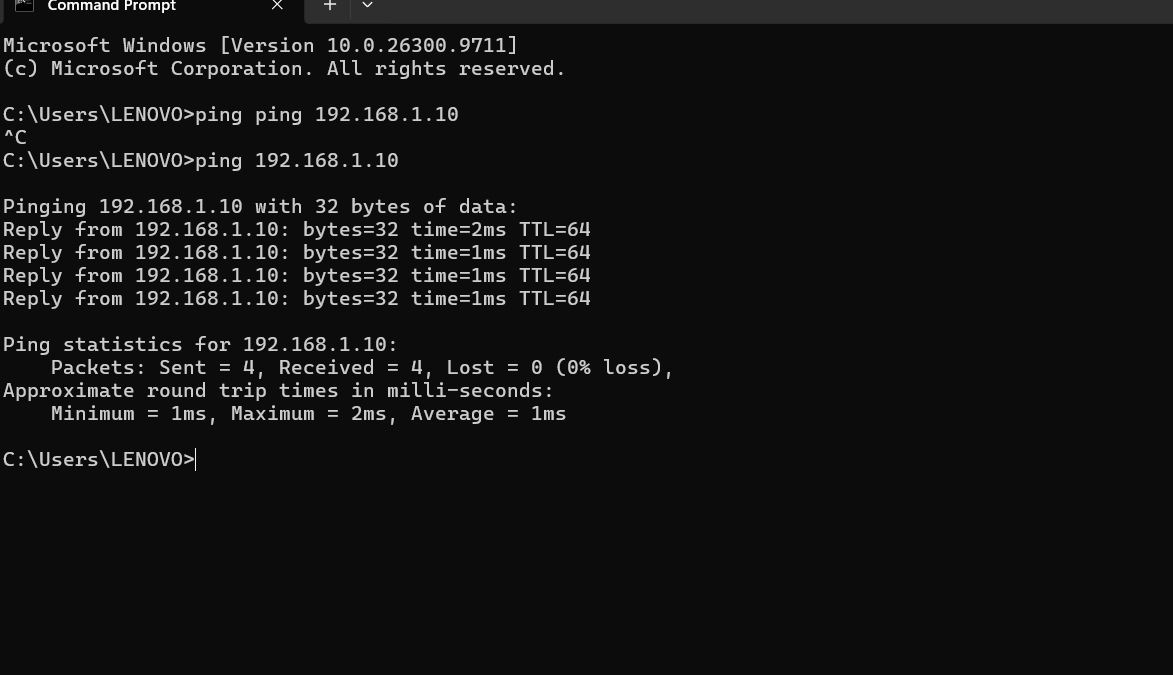
\includegraphics[width=0.96\linewidth,height=0.29\textheight,keepaspectratio]{../assets/images/pingingSDR.png}
\caption{\rtl{خروجی ثبت‌شدهٔ آزمون شبکه}}\label{fig:ping}
\end{figure}
\clearpage
\section{\rtl{مسیر الف؛ MATLAB}}
\rp{شکل \ref{fig:matlab} کد دریافت و پنجرهٔ تحلیل‌گر را نشان می‌دهد. تنظیمات خوانده‌شده در جدول \ref{tab:matlab} ثبت شده‌اند.}
\begin{table}[H]\centering
\renewcommand{\arraystretch}{1.2}
\begin{tabular}{|p{0.55\linewidth}|p{0.32\linewidth}|}\hline
\rtl{\lr{ip:192.168.1.10}} & \rtl{نشانی اتصال} \\ \hline
\rtl{\lr{945 MHz}} & \rtl{فرکانس مرکزی} \\ \hline
\rtl{\lr{2.6 MS/s}} & \rtl{نرخ نمونه‌برداری} \\ \hline
\rtl{\lr{Manual / 20 dB}} & \rtl{حالت و بهرهٔ گیرنده} \\ \hline
\rtl{\lr{4096}} & \rtl{نمونه در هر فریم} \\ \hline
\rtl{ثبت نشده} & \rtl{نسخهٔ MATLAB} \\ \hline
\rtl{ثبت نشده} & \rtl{سریال دستگاه} \\ \hline
\rtl{ثبت نشده} & \rtl{سفت‌افزار} \\ \hline
\rtl{ثبت نشده} & \rtl{بازهٔ فعال} \\ \hline
\end{tabular}
\caption{\rtl{تنظیمات MATLAB و فیلدهای تکمیلی}}\label{tab:matlab}\end{table}
\begin{figure}[H]
\centering
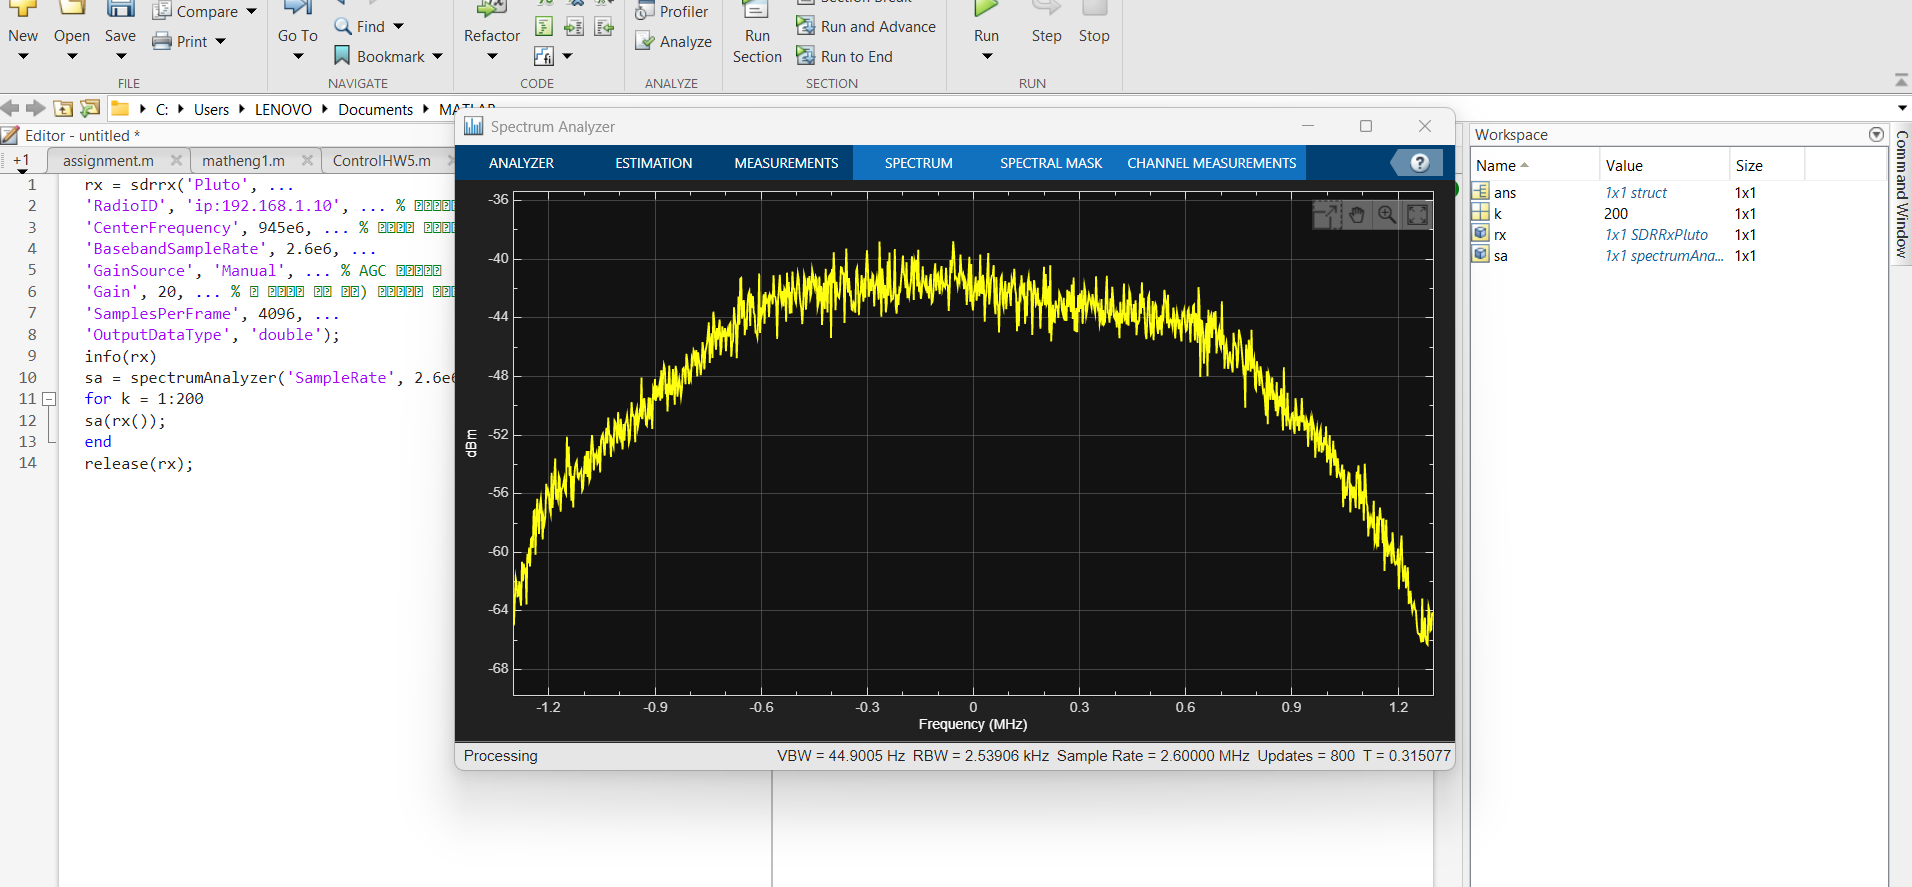
\includegraphics[width=0.96\linewidth,height=0.29\textheight,keepaspectratio]{../assets/images/MATLAB1.png}
\caption{\rtl{محیط MATLAB و اجرای کد دریافت}}\label{fig:matlab}
\end{figure}
\clearpage
\section{\rtl{مسیر ب؛ GNU Radio و نرم‌افزارهای ویندوز}}
\rp{نسخهٔ محیط در شکل \ref{fig:gnu} و پنجرهٔ طیف در شکل \ref{fig:grspec} مستند شده‌اند. فایل اصلی فلوگراف در ورودی موجود نبود. جدول \ref{tab:windows} اطلاعات قابل‌خواندن را ثبت می‌کند.}
\begin{table}[H]\centering
\renewcommand{\arraystretch}{1.2}
\begin{tabular}{|p{0.55\linewidth}|p{0.32\linewidth}|}\hline
\rtl{\lr{3.10.12.0}} & \rtl{نسخهٔ GNU Radio} \\ \hline
\rtl{\lr{3.12.9}} & \rtl{نسخهٔ Python همراه} \\ \hline
\rtl{\lr{SDR++ 1.3.2 / SDRangel 8.0.0}} & \rtl{نرم‌افزارهای آماده} \\ \hline
\rtl{\lr{96 MHz}} & \rtl{فرکانس نمایشی در SDRpp\_2} \\ \hline
\rtl{\lr{45 dB}} & \rtl{بهره در SDRpp\_2} \\ \hline
\rtl{\lr{(usb)}} & \rtl{مسیر نمایش‌داده‌شده در SDRpp\_2} \\ \hline
\rtl{\lr{90 MHz}} & \rtl{فرکانس در SDR\_angle1} \\ \hline
\end{tabular}
\caption{\rtl{ثبت اطلاعات مسیر ویندوز}}\label{tab:windows}\end{table}
\rp{دستورکار، فرکانس ۹۴۵ مگاهرتز و بهرهٔ دستی حداکثر ۳۰ دسی‌بل با آنتن را تعیین می‌کند. توضیح انتخاب تنظیمات ثبت‌شده و پاسخ به معیار پذیرش، در بخش تحلیل توسط تیم تکمیل می‌شود.}

\begin{figure}[H]
\centering
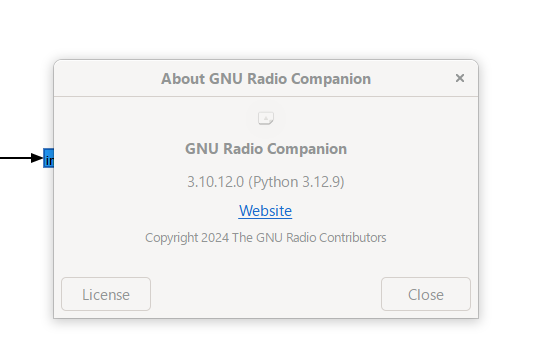
\includegraphics[width=0.96\linewidth,height=0.17\textheight,keepaspectratio]{../assets/images/gnuRadoWindowsVersion.png}
\caption{\rtl{پنجرهٔ نسخهٔ GNU Radio Companion}}\label{fig:gnu}
\end{figure}
\begin{figure}[H]
\centering
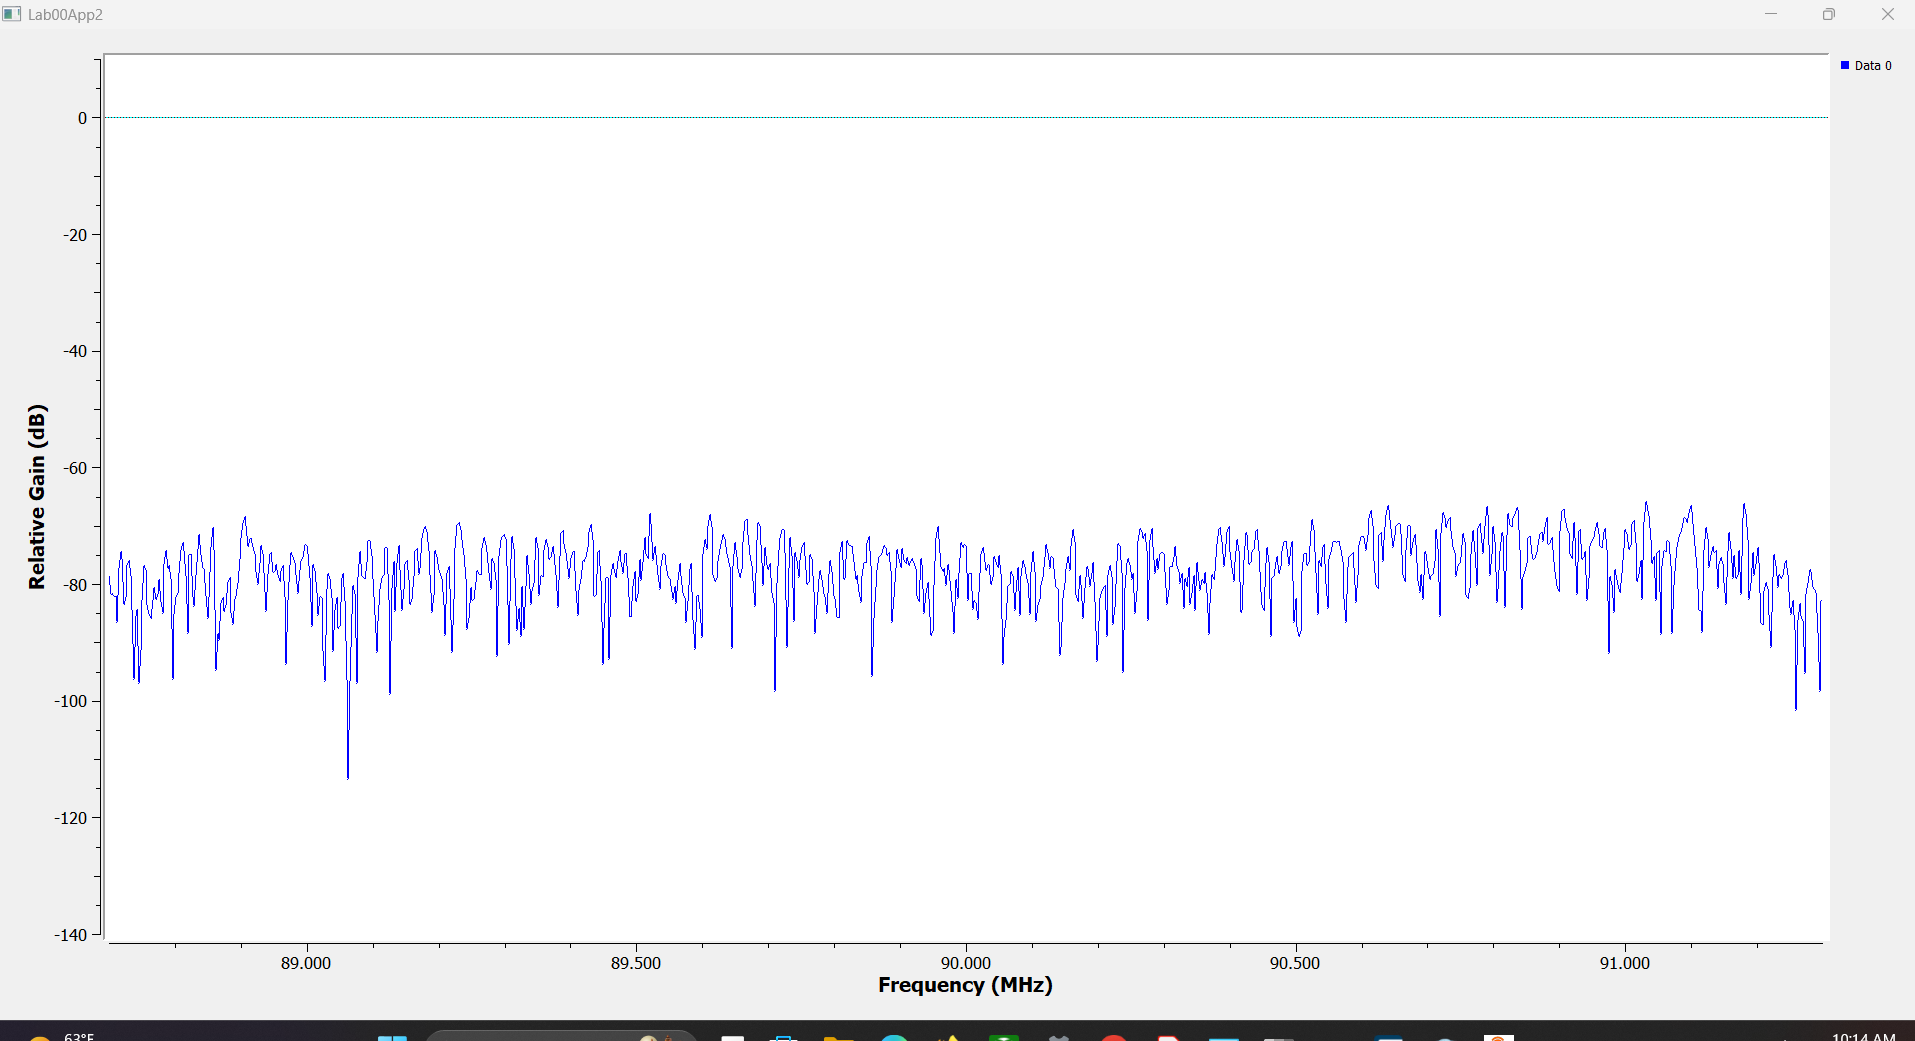
\includegraphics[width=0.96\linewidth,height=0.29\textheight,keepaspectratio]{../assets/images/GNUradioWindows_Spectrum.png}
\caption{\rtl{پنجرهٔ طیف در GNU Radio ویندوز}}\label{fig:grspec}
\end{figure}
\clearpage
\rp{شکل‌های \ref{fig:sdpp} و \ref{fig:angle} تصاویر دو نرم‌افزار آماده را نشان می‌دهند. این تصاویر به‌خودی‌خود تأیید انجام آزمون خواسته‌شده در دستورکار نیستند.}
\begin{figure}[H]
\centering
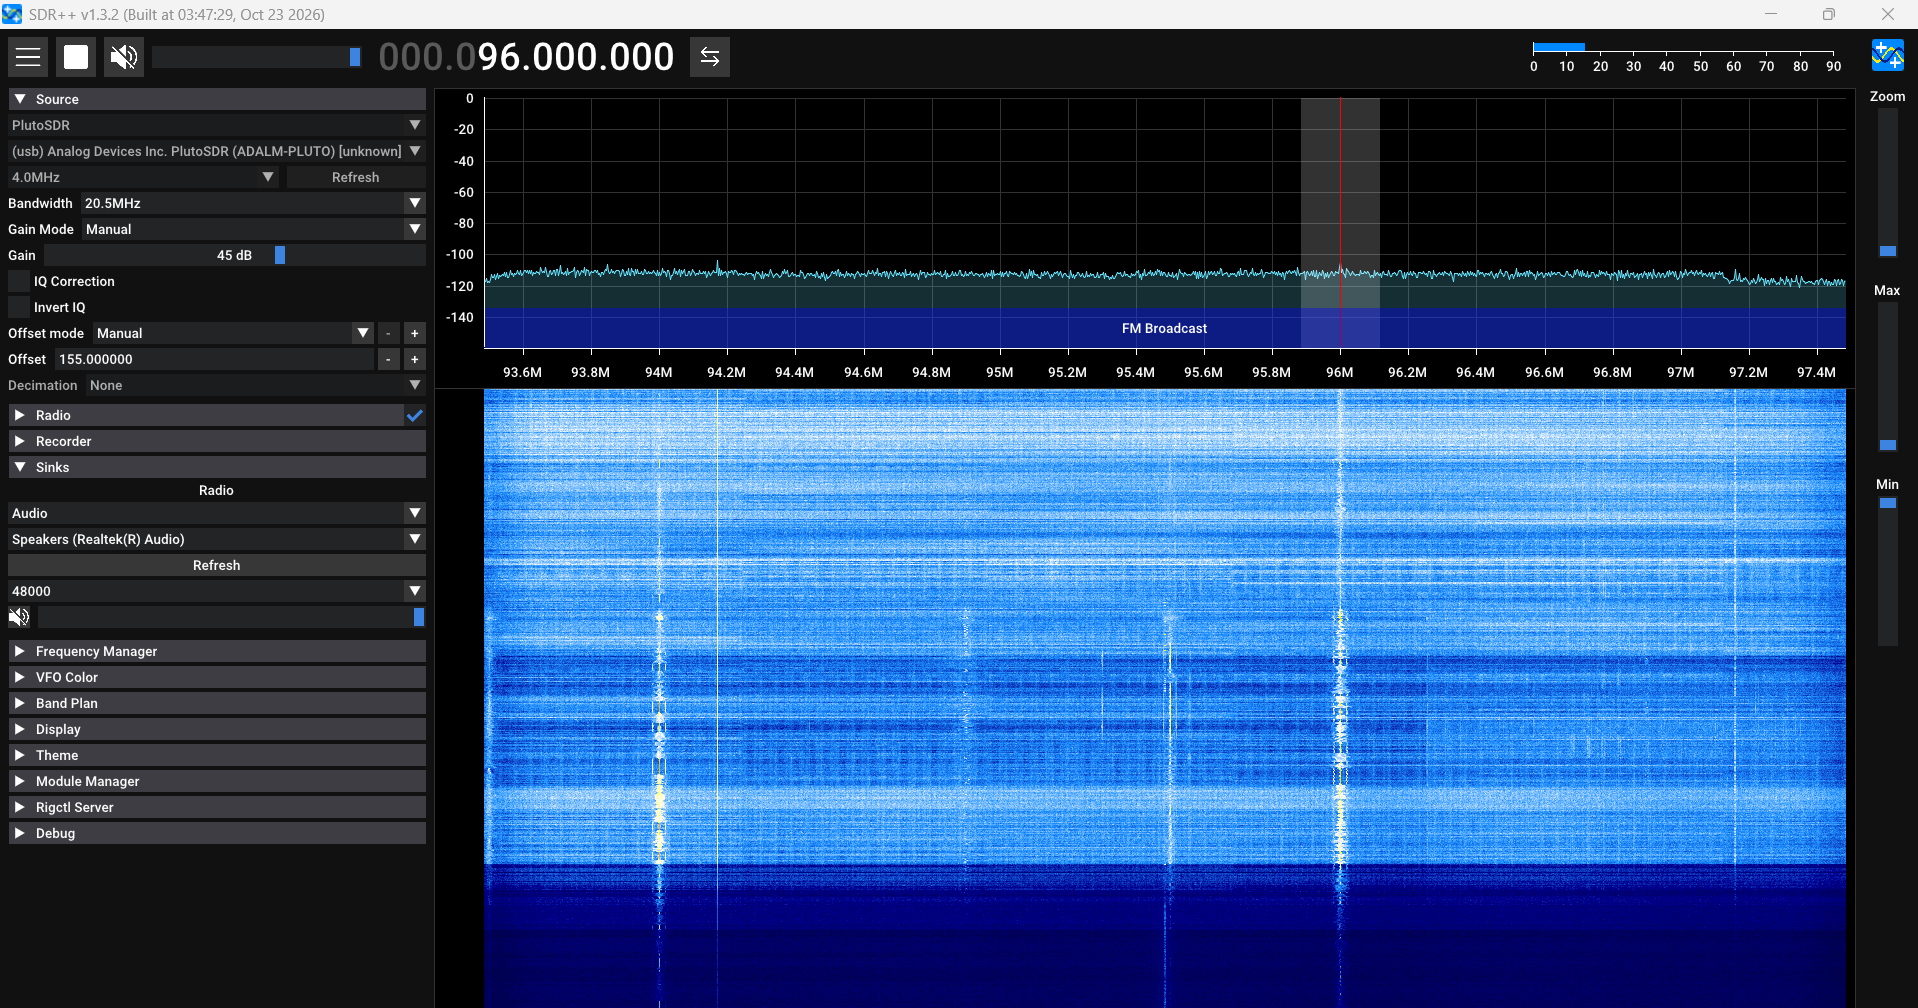
\includegraphics[width=0.96\linewidth,height=0.29\textheight,keepaspectratio]{../assets/images/SDRpp_2.png}
\caption{\rtl{رابط SDR++ و تنظیمات ثبت‌شده}}\label{fig:sdpp}
\end{figure}
\begin{figure}[H]
\centering
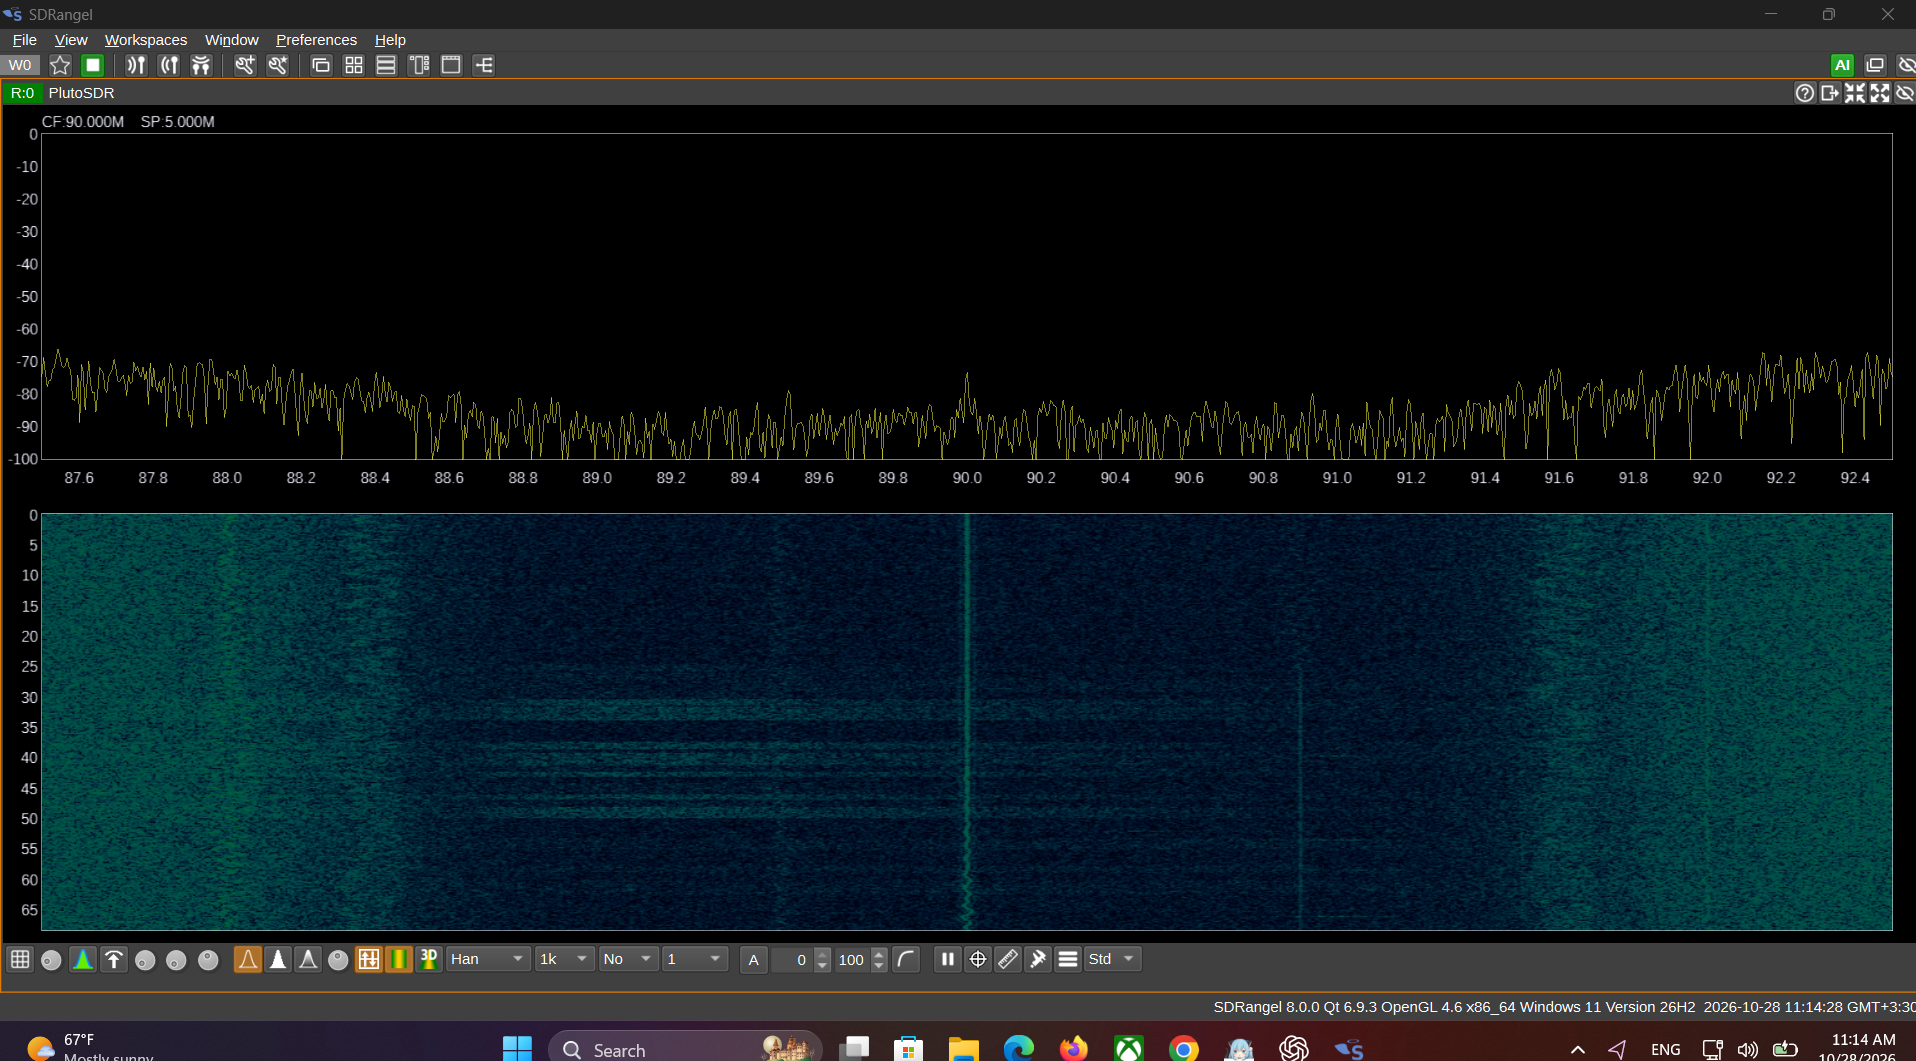
\includegraphics[width=0.96\linewidth,height=0.29\textheight,keepaspectratio]{../assets/images/SDR_angle1.png}
\caption{\rtl{رابط SDRangel و تنظیمات ثبت‌شده}}\label{fig:angle}
\end{figure}
\clearpage
\section{\rtl{مسیر ج؛ اوبونتو}}
\begin{quote}\rp{\textbf{ثبت مسیر اوبونتو؛ در انتظار نوشتهٔ تیم.} در فایل‌های ورودی، مدرکی از این مسیر وجود ندارد. نسخهٔ اوبونتو، نسخهٔ GNU Radio، خروجی iio\_info، تصویر GRC و آزمون ابزار اضافی باید افزوده شوند.}\end{quote}
\section{\rtl{مسیر د؛ پایتون}}
\rp{خروجی قابل‌خواندن ترمینال در شکل \ref{fig:python} برابر \lr{samples: (4096,) sample\_rate: 2600000} است. جدول \ref{tab:python} تنظیمات کد را ثبت می‌کند.}
\begin{table}[H]\centering
\renewcommand{\arraystretch}{1.2}
\begin{tabular}{|p{0.55\linewidth}|p{0.32\linewidth}|}\hline
\rtl{\lr{ip:192.168.1.10}} & \rtl{نشانی اتصال} \\ \hline
\rtl{\lr{945 MHz}} & \rtl{فرکانس مرکزی} \\ \hline
\rtl{\lr{2.6 / 2 MHz}} & \rtl{نرخ نمونه / پهنای باند} \\ \hline
\rtl{\lr{manual / 20 dB}} & \rtl{حالت و بهرهٔ گیرنده} \\ \hline
\rtl{\lr{4096}} & \rtl{اندازهٔ بافر} \\ \hline
\rtl{ثبت نشده} & \rtl{نسخهٔ pyadi-iio} \\ \hline
\rtl{مسیر ترمینال شامل \lr{radioconda} است} & \rtl{محیط اجرا} \\ \hline
\end{tabular}
\caption{\rtl{تنظیمات قابل‌خواندن پایتون}}\label{tab:python}\end{table}
\begin{figure}[H]
\centering
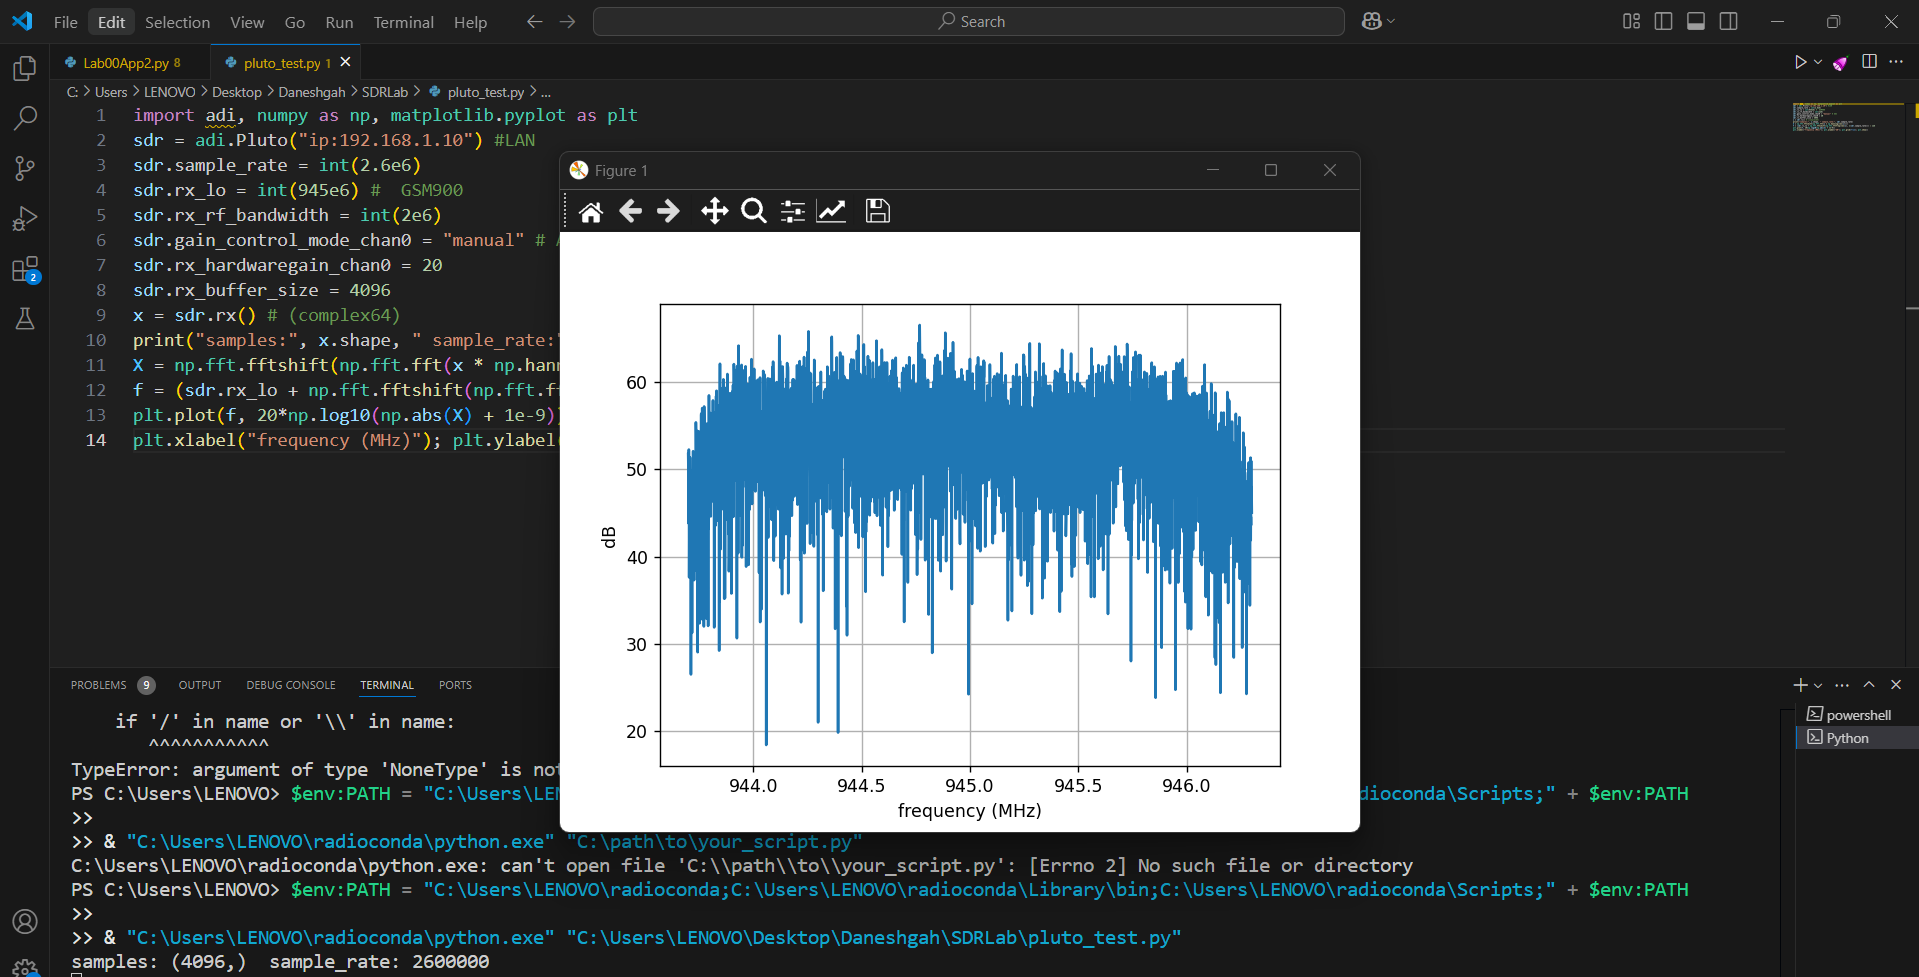
\includegraphics[width=0.96\linewidth,height=0.29\textheight,keepaspectratio]{../assets/images/Python_output.png}
\caption{\rtl{اسکریپت، نمودار و خروجی ترمینال در VS Code}}\label{fig:python}
\end{figure}
\clearpage
\section{\rtl{وضعیت آمادگی و داده‌های خام}}
\rp{جدول \ref{tab:ready} وضعیت مدارک را بر اساس جدول ۱۰ دستورکار نشان می‌دهد. این جدول جای امضای دستیار را نمی‌گیرد.}
\begin{table}[H]\centering
\renewcommand{\arraystretch}{1.2}
\begin{tabular}{|p{0.55\linewidth}|p{0.32\linewidth}|}\hline
\rtl{تصویر پاسخ موجود؛ تصویر IPv4 لازم است} & \rtl{شبکه} \\ \hline
\rtl{تصویر اجرا موجود؛ مشخصات دستگاه لازم است} & \rtl{الف} \\ \hline
\rtl{تصاویر موجود؛ فلوگراف و ثبت آزمون نهایی لازم است} & \rtl{ب} \\ \hline
\rtl{مدرک ارائه نشده} & \rtl{ج} \\ \hline
\rtl{تصویر خروجی موجود؛ نسخه و فایل خام لازم است} & \rtl{د} \\ \hline
\end{tabular}
\caption{\rtl{وضعیت مدارک آمادگی}}\label{tab:ready}\end{table}
\rp{فایل خام I/Q، فایل اصلی GRC، کد اصلی جلسه و لاگ کامل همراه ورودی نبودند. هیچ عددی برای توان، SNR یا کیفیت دریافت از روی تصاویر استخراج نشده است. اسکرین‌شات رابط نرم‌افزار فقط به‌عنوان مدرک رابط نگه داشته شده است؛ نمودار علمی نهایی باید از دادهٔ خام و ترجیحاً به‌صورت برداری تولید شود.}

\section{\rtl{تحلیل و عیب‌یابی}}
\begin{quote}\rp{\textbf{تحلیل نتایج؛ در انتظار نوشتهٔ تیم.} اعضای تیم توضیح خود را دربارهٔ معیار پذیرش، تنظیمات و شواهد هر مسیر می‌نویسند. ادعاهای عددی باید به فایل خام مشخص متصل باشند.}\end{quote}
\begin{quote}\rp{\textbf{عیب‌یابی؛ در انتظار نوشتهٔ تیم.} نشانهٔ خطا، اقدام واقعی و نتیجهٔ آزمون مجدد را از لاگ جلسه وارد کنید.}\end{quote}
\section{\rtl{نتیجه‌گیری}}
\begin{quote}\rp{\textbf{جمع‌بندی؛ در انتظار نوشتهٔ تیم.} اعضای تیم جمع‌بندی خود را دربارهٔ آزمون‌های انجام‌شده، مدارک موجود و کارهای باقی‌مانده می‌نویسند.}\end{quote}
\section{\rtl{اعلام استفاده از هوش مصنوعی}}
\rp{در تهیهٔ این نسخه از ChatGPT برای ساخت قالب HTML/CSS و LaTeX، ویرایش نگارشی، سامان‌دهی تصاویر، رونویسی تنظیمات قابل‌خواندن و آماده‌کردن قالب کد استفاده شده است. بخش‌های تحلیل، تفسیر داده و نتیجه‌گیری در این نسخه خالی مانده‌اند تا اعضای تیم آن‌ها را بنویسند. مسئولیت بررسی نهایی با اعضای تیم است.}

\begin{minipage}{\linewidth}
\small
\bibliographystyle{plainnat}
\bibliography{references}
\end{minipage}
\end{document}
